\section{Evaluation}
\label{eval}

% eval figures all in one big table
\begin{figure*}[t!]
\centering
\begin{tabular}{ccc}
    \tablefigure{MPI-IO Test on PanFS}{panfs}
    &
    \tablefigure{MPI-IO Test on GPFS}{gpfs}
    &
    \tablefigure{MPI-IO Test on Lustre}{lustre}
    \\
    \tablefigure{LANL Anonymous 1}{lanl1}
    &
    \tablefigure{LANL Anonymous 2}{lanl2}
    &
    \tablefigure{LANL Anonymous 3}{lanl3}
    \\
    \tablefigure{PatternIO}{pattern}
    &
    \tablefigure{QCD}{qcd}
    &
    \tablefigure{BTIO}{btio}
    \\
    \tablefigure{FLASH IO}{flash}
    &
    \tablefigure{SUMMARY}{summary}
    &
    \tablefigure{Chombo IO}{chombo}
\end{tabular}
\mycaption{fig-eval}{Experimental Results.}{
The three graphs in the top row are the same graphs that were presented
earlier in Figure~\ref{fig-motivation}, except now they have an additional
line showing how PLFS allows an N-1 checkpoint to achieve most, if not all,
of the bandwidth available to an N-N checkpoint. 
The bar graph in the center of the bottom row consolidates these results and
shows a pair of bars for each, showing both the relative minimum and the
maximum speedups achieved across the set of experiments.  Due to radically
different configurations for these various experiments, the axes for 
these graphs are not consistent.  The relative comparison within each graph
should be obvious; absolute values can be ascertained by reading the axes.
}
\end{figure*}


We present the results of our experimental evaluation in Figure~\ref{fig-eval}.
Eleven of these twelve graphs present one experiment each. The twelfth,
Figure~\ref{eval:summary}, presents a summary. In the majority of these graphs,
the write bandwidth is shown on the \yaxis\ in \MBs\ as a function of the
number of processes. We will note it in the text for those few graphs for
which we deviate from this general configuration. The write bandwidth that we
report is whatever is reported by the particular benchmark; whenever possible,
we report the most conservative value (\ie\ we include open and close times in
our write times, and we either barrier after close or we use the time reported
by the slowest writer). Finally we have attempted to run multiple iterations
for each experiment; where applicable, the standard deviation is therefore
included.

\subsection{MPI-IO Test}

The top three graphs, 
Figures~\ref{eval:panfs},~\ref{eval:gpfs},~and~\ref{eval:lustre}, present the
results of our study using the LANL synthetic checkpoint tool, \Term{MPI-IO
Test}~\cite{mpi-io-test}, on three different parallel file systems, PanFS, GPFS,
and Lustre. 
There are several things to notice in these graphs. The first is that these
are the same three graphs that we presented in Figure~\ref{fig-motivation}
except that we have now added a third line to each. The three lines show the
bandwidth achieved by writing an N-N pattern directly to the \upfs, the
bandwidth achieved by writing an N-1 pattern directly to the \upfs, and the
third line is the bandwidth achieved by writing an N-1 pattern {\em indirectly}
to the \upfs\ through \plfs.

These graphs illustrate how the performance discrepancy between N-N
and N-1 checkpoint patterns is common across PanFS, GPFS,
and Lustre. Remember, as was discussed in Section~\ref{motivation}, switching
to N-N is not a viable option for many applications which are inextricably wed
to an N-1 pattern and are resigned to the attendant loss of bandwidth.
Fortunately, as is evidenced by these graphs, \plfs\ allows these applications
to retain their preferred N-1 pattern while achieving most, if not all, of the
bandwidth available to an N-N pattern. Particularly for the PanFS results,
which were run on our Roadrunner supercomputer, \plfs\ achieves the full
bandwidth of an N-N pattern (\ie\ up to about 31 \GBs). In fact, for several
of the points, an N-1 pattern on \plfs\ actually outperforms an N-N pattern
written directly to PanFS. Although we have yet to fully investigate the exact
reason for this, there are several reasons why this could be the case. The
first is that \plfs\ rearranges writes into a log structured pattern so an N-N
pattern which incurs seeks could do worse than a \plfs\ pattern which appends
only. Secondly, the structure of the \plfs\ container spreads data across
multiple sub-directories within a top-level directory whereas a typical N-N
pattern confines all N files into only a single parent directory.

Although \plfs\ does improve the bandwidth of N-1 patterns on GPFS and Lustre,
the improvement is not as large as it is on PanFS. This is because the scale of
the experiments on PanFS are 200 times larger than on the other two platforms.
In the inset in Figure~\ref{eval:panfs} at the extreme low values for the
number of processes, we see that \plfs\ does not scale N-1 bandwidth as fast as
N-N scales for PanFS as well. This is due to overheads incurred by both FUSE
and \plfs; these overheads limit the total bandwidth achieved by any single
compute node relative to N-N. For HPC systems at extreme scale this limitation
does not matter since aggregate bandwidth across multiple nodes is more
relevant than the bandwidth from a single node. In this case the real limiting
factor is the total bandwidth capacity of the storage fabric, which generally
saturates when using only a small fraction of compute nodes.  However, with
poorly-behaved IO patterns (\ie\ N-1), even very large jobs may not reach these
bandwidth limits because they will be more severely constrained by file system
limitations as exemplified by Figure~\ref{fig-motivation}. \plfs\ is designed
to remove these file system limitations, so that jobs can achieve higher
bandwidth and reach the same limitation of the storage fabric which is
constraining N-N bandwidth.  We will examine the FUSE and PLFS overheads in
greater detail in Section~\ref{overhead}. 
 
An unusual feature of the inset graph in Figure~\ref{eval:panfs} is that there
are localized bottlenecks about 700 processes.  This is due to the architecture
of Roadrunner and it's connection to its 1000 blade PanFS storage system.
Roadrunner is split into seventeen sub-clusters, \Term{CUs}, each of which can
run 720 proceses.  The CUs are fully connected via an Infiniband fat tree,
however, in order to minimize network infrastructure costs, the storage system
is partitioned into multiple sub-nets. Each CU currently has six specialized IO
nodes, one for each sub-net; these six IO nodes are the storage bandwidth
bottleneck.  Therefore, as a job grows within a CU, it quickly saturates the IO
node bandwidth; when it grows into another CU, its bandwidth increases sharply
due to gaining six additional IO nodes: this explains the ``stair-step"
behavior of the N-N and \plfs\ lines in this graph. 
 
We do see this same behavior in our GPFS and Lustre graphs, but due to the
very small size of our test systems, we do not have enough compute nodes to
saturate the available storage bandwidth and thus neither the N-N nor the
\plfs\ lines in these graphs reach a storage bandwidth bottleneck. 

\subsection{Real LANL Applications}

The second row in Figure~\ref{fig-eval} shows the results of using \plfs\ to
improve the bandwidth of three important LANL applications which use N-1
checkpoint patterns. The application shown in Figure~\ref{eval:lanl1} is the
application whose developers augmented their checkpoint routine with a new
checkpoint library called bulkio, which aggregates and buffers writes into
larger, contiguous writes more friendly to the \upfs. Therefore we compare the
bulkio method writing directly to PanFS to the old MPI-IO method writing
indirectly to PanFS via \plfs.  This data was collected on Roadrunner.  The
next two graphs show similar results; using \plfs\ to rearrange an N-1 pattern
yields significantly improved bandwidths.  Figure~\ref{eval:lanl2} was run on a
small \rrz\ which consists of 128 8-core compute nodes with a 66 blade PanFS
storage system, whereas Figure~\ref{eval:lanl3} was run on Roadrunner itself.
Note that these are extremely important applications at LANL; it has been
estimated that they account for more than half of the total computing cycles at
LANL.  Although these applications must remain anonymous, traces of their IO
are available~\cite{plfs-maps}.

\subsection{NERSC's PatternIO Benchmark}

Figure~\ref{eval:pattern} presents the data derived from our measurements taken
using NERSC's PatternIO benchmark~\cite{nersc} which plots write bandwidth as a
function of \syscall{write} size. Notice that this deviates from the other
graphs in Figure~\ref{fig-eval} which plot write bandwidth as a function of the
number of processes. For this experiment, run on the \rrz, the number of
processes was set at a constant 512. This graph also is a scatter plot instead
of using lines with standard deviations. The points for writing directly to
PanFS show three interesting slopes all converging at about 1 GB/s on the far
right side of the graph. The highest of these three regions shows the
performance of \syscall{writes} when the write size is both block aligned and
aligned on file system boundaries. The middle region is when the write size is
block aligned only and the lowest region is when the write size is not aligned
at all. {\em This graph demonstrates that \plfs\ allows an application to
achieve a consistently high level of write bandwidth regardless of the size, or
alignment, of its \syscall{writes}.}

\subsection{Other Benchmarks}

The remainder of the graphs show various other parallel IO benchmarks with an
N-1 checkpoint pattern. QCD~\cite{qcd-io} in Figure~\ref{eval:qcd} shows a
large improvement using \plfs\ but this improvement actually {\em degrades} as
the number of processes increases. This is because the amount of data written
by QCD is a small constant value and the overhead due to container creation
incurred in the \syscall{open} becomes proportionally greater as the amount of
data written by each process decreases. BTIO~\cite{btio-io} in
Figure~\ref{eval:btio} also shows a large improvement but only
for one data point.
FLASH~IO~\cite{flash-io} and Chombo~IO\cite{chombo-io}, shown respectively in
Figures~\ref{eval:flash}~and~\ref{eval:chombo}, both show improvement due to
\plfs\ which scales nicely with an increasing number of processes. FLASH was
run on Roadrunner whereas Chombo was run on the \rrz; both were built with the
HDF5 library~\cite{hdf5}.

\subsection{Summary}

A summary of the benchmark results, excluding the LANL and NERSC synthetics, is
presented in Figure~\ref{eval:summary}. This summary shows a pair of bars for
each benchmark; one for both the worst-case and best-case speedups for \plfs.
Only in one case did \plfs\ actually degrade performance: a slowdown of three
percent for LANL 1 when it was run on just a single node. Although we did test
on single nodes to be thorough, single node sized jobs are extremely rare in
HPC. The relevant results from reasonably sized jobs, showed at least a
doubling of performance for all studied benchmarks. QCD and BTIO experienced a
single order of magnitude improvement. The best result was observed for FLASH
which was improved in the best case by two orders of magnitude. 

\subsection{Overhead}
\label{overhead}

\begin{SCfigure}
    \centering
    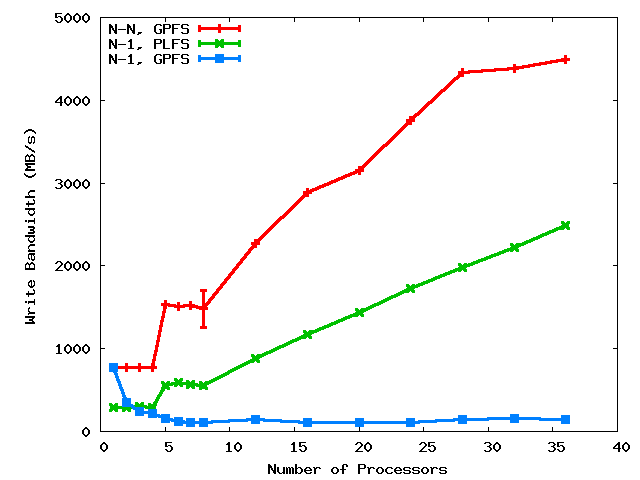
\includegraphics[width=0.4\textwidth]{data/overhead/gpfs.eps}
    \mycaption{fig-overhead}{Overhead.}{
        Ideally, N-1
        patterns written through \plfs\ would be able to 
        achieve the bandwidth available to an N-N pattern
        written directly to the \upfs.  However, 
        this graph shows that various overheads make this
        difficult.  Even though
        there is overhead, the important
        point is that \plfs\ still allows an N-1 pattern to
        be written much more quickly than if it was written
        directly to the \upfs. 
        \vspace{.5cm}
    }
\end{SCfigure}


As was seen in
Figures~\ref{eval:panfs},~\ref{eval:gpfs},~and~\ref{eval:lustre}, N-1 patterns
written through \plfs\ only match the bandwidth achieved by N-N patterns
written directly to the \upfs\ once the storage system bandwidth is saturated.
For small number of processes, \plfs\ cannot match the performance of N-N
(nonetheless, it does still improve bandwidth over a direct N-1 pattern). This
overhead is measured in Figure~\ref{fig-overhead} which shows results as
measured on LANL's GPFS system. In order to measure the both overhead incurred
by FUSE as well as any additional overhead incurred by \plfs, we developed a
second FUSE file system, \Term{\noopfs}.  \noopfs\ does no extra work, merely
redirecting all IO to the \upfs (\ie\ GPFS). For those readers familar with
FUSE, please note that \noopfs\ caches the file descriptor created in the
\syscall{open} into the opaque FUSE file handle pointer, uses it for subsequent
\syscall{writes} and \syscall{reads}, and closes it in the \syscall{flush}.

Figure~\ref{fig-overhead} is almost the same as Figure~\ref{eval:gpfs} which
compares the bandwidths measured for N-N directly to GPFS, N-1 directly to
GPFS, and N-1 indirectly to GPFS written through \plfs. The difference here is
that several new measurements have been added. The first is for N-N written
indirectly to GPFS through \noopfs. This line is significantly lower than the
line for N-N written directly to GPFS; the delta between these lines is the
overhead incurred due to FUSE, which is approximately 20\%. The next
measurement added is running an N-N workload through \plfs; this shows the
additional overhead incurred by \plfs, approximately 10\%. 
The delta beween that line and the existing N-1 through \plfs\
measurements show additional overhead which we believe is due to serializations
within FUSE due to multiple processes accessing the same path within FUSE's
file table (approximately another 10\% loss). For completeness, we also
measured the bandwidth achieved by an N-1 workload written through \noopfs;
therefore, the bottom two lines on the graph provide another view of the
overhead lost to FUSE.

Although this graph shows a total overhead cost of about 40 to 50\%, this loss
of potential bandwidth is not unduly concerning. As was seen in
Figure~\ref{eval:panfs}, the loss of potential bandwidth due to this overhead
disappears for reasonable HPC processor counts. Even with a limited per-node
bandwidth, a relatively small number of nodes writing through \plfs\ is able to
saturate the storage bandwidth. 


\subsection{Beyond Writing}
Although \plfs\ is designed primarily for {\em writing} checkpoints,
checkpoint files are still occassionally read.
We must therefore weigh improvements in 
write bandwidth against possible degradations in other operations. 

\subsubsection{Read Bandwidth}
\begin{figure*}[tb]
    \centering
        \readgraph{Uniform Restart}{nn}{data/reads/nn.eps}
        \readgraph{Non-uniform Restart}{nm}{data/reads/nm.eps}
        \readgraph{Archive Copy}{n1}{data/reads/archive.eps}
    \\
    \mycaption{fig-reading}{Read Bandwidth.}{
These three graphs show the results of our read measurements on the
\rrz. We created a set 20~\GB\ N-1 checkpoint files through
\plfs\ and another directly on PanFS.  Each file was produced by a different
number of writers; all of the \syscall{writes} were 47001 bytes in size.  For
each graph, the \yaxis\ shows the read bandwidth as a function of the number of
writers who created the file.  The graph on the left shows the read bandwidth
when the number of readers is the same as the number of writers, as is the case
in a typical uniform restart; in this case, the size of the reads is the same
as the size of the original writes.  The graph in the middle emulates a
non-uniform restart in which the application resumes on one fewer compute
nodes; in this case, the size of the \syscall{reads} is slightly larger than
the size of the original \syscall{writes}.  Finally, the graph on the right
shows the read bandwidth when there only four readers; we used LANL's archive
copy utility and modelled the common scenario of copying checkpoint data to an
archive system using a relatively small number of readers.  To enable
comparison across graphs, the axis ranges are consistent.
} 

\end{figure*}



To ensure \plfs\ does not improve write bandwidth at the expense of read
bandwidth, we ran a set of read experiments on \rrz\ which are shown in
Figure~\ref{fig-reading}. We first created two sets of 20~\GB\ files, each
written by a different number of writers; all writes were 47001 bytes (in other
words, increasing numbers of writers issued decreasing numbers of writes). One
set was created directly on PanFS; the other indirectly through \plfs. In all
cases, reads were performed on different nodes than those where the
corresponding data was written and caches were always flushed between
successive reads.

We measured the time to read these files using three different read
scenarios. One emulates a \Term{uniform restart} in which the number of
processes resuming the application is the same as the number that wrote the
last checkpoint. In this case, each process within the parallel job reads the
same data in the same order as one of the previous writers. In
contrast, a \Term{non-uniform restart} is one in which the number of
readers is different from the number of writers and the read offsets are
therefore not aligned with the previous writes. In this case, we emulate the
scenario where an application resumes after a failure by simply running on the
newly reduced number of nodes. The number of reads is not affected by the size
of the job for typical N-1 checkpoints. Each read is extracting a region for a
particular variable within the simulation. The size of this region depends on
the number of processes within the job. Each gets $1/Nth$ of the region.
Specifically, for a non-uniform restart in which the number of processes, $N$,
has been reduced by $M$, the size of each read will be $N/(N-M)$ times the size
of the original writes. The third read scenario we emulated is a typical
scenario in which a relatively, small fixed number of processes reads a
checkpoint in order to save it onto an archive system. For these measurements,
we used LANL's archive copy utility with fours readers each running on their
own node; each reader read just one contiguous 5~\GB\ region by issuing 
sequential 1~\MB\ reads. 

\if 0
% tempting to say this but we said at the beginning that we wouldn't really
% talk about segmented anymore
The archive copy uses an N-1 segmented pattern to
read a checkpoint that was written with N-1 strided.
\fi

The results of these experiments can be seen in Figure~\ref{fig-reading}. In
order to allow comparison across the three experiments, the ranges of the axes
have been made consistent. The \yaxis\ shows read bandwidth as a function of
the number of writers who created the checkpoint. We can easily see from these
graphs that the highest bandwidth is achieved using \plfs\ in the uniform
restart scenario. This is not surprising: each reader moves sequentially
through just one, nonshared file, a pattern easily improved through prefetching
performed by the \upfs. The bandwidth decreases here due to the decreasing
amount of data read as the number of readers increases. With less data read by
each, the open times begin to dominate, and there is less potential for
prefetching. The very low bandwith observed when the checkpoint is stored
directly on PanFS is also not surprising due to its layout of data within RAID
groups. Each contiguous \GB\ is spread only across a single RAID group (in this
case consisting of just eight storage devices from a pool of around one
hundred). The nature of the N-1 pattern and the size of the reads means that
all readers will almost always be reading within just a single RAID group. In
addition to limiting the bandwidth to only a few storage devices, it also
reduces the bandwidth from each of them due to overloading them with
non-sequential requests.

The results for the non-uniform restart can be similarly explained. The PanFS
results and explanation are essentially the same. The results for \plfs\ are
also very similar; better than PanFS due to spreading the reads across all
storage devices and not quite as good as the \plfs\ results for the uniform
restart. The difference between the uniform and non-uniform results for \plfs\
is only seen for small numbers of readers in the area where \plfs\ was helped
by prefetch in the uniform experiment. Since the readers are reading different
offsets than were written in the non-uniform restart, they will read multiple
data files instead of just reading a single one. The \upfs, unsurprising,
does not identify this admittedly strange pattern and therefore there is no
prefetch benefit. Only when there is no longer any prefetch benefit, 
do these results converge.

Although we are pleased to see that \plfs\ also does relatively well for the
archive copy experiment, we do not yet fully understand all of these results.
We can think of no reason why the bandwidths should be this low and we assumed
that PanFS would easily outperform \plfs\ due to having contiguous data within
its RAID groups instead of having data spread across multiple data files
within a \plfs\ container.  However, we are not surprised to see the read
bandwidths drop as the number of writers increases.  Increasing numbers of
writers results in a data layout with fewer large contiguous regions of data
for both \plfs\ and PanFS; therefore, the read bandwidth will suffer
accordingly.

%this behavior has been
%independently observed thrice that we know of: once by us, and twice by two
%groups of students at CMU. 

\subsubsection{Metadata Queries}

As we discussed in Section~\ref{arch-meta}, there are currently two techniques
used to discover the metadata for a \plfs\ file. For a file being currently
written, metadata is discovered by \syscall{stat'ing} individual data files.
When a file is closed, metadata information is cached as file names within a
specific subdirectory inside the container. Thereafter, metadata information
can be discovered merely by issuing a \syscall{readdir}. Obviously, the first
technique is much slower; if our primary interest was in optimizing metadata
query rates, than we could cache this metadata following every write. However,
since \plfs\ is designed for checkpoint writing, we do not consider this
technique.

Figure~\ref{fig-metadata} compares these two times against the time it takes to
query a closed file written directly to the \upfs, PanFS. We have not yet
measured the time to query an open file on PanFS. For this experiment,
conducted on LANL's \rrz, we created two sets of 20~\GB\ files each written by
a different number of writers all issuing 47001 byte-sized writes. One set was
created directly on PanFS; the other indirectly through \plfs.  As the graph
shows, the \syscall{stat} times for closed files on \plfs\ and PanFS are
approximately the same.  However, as expected, the time to query a \plfs\ file
open for writing is greater than to query a closed file.

%plateaus for \plfs may be due to \Term{statahead} in the PanFS client.
%We suspect this is due to the small number of writers available on
%the \rrz; we hope to rerun this experiment on Roadrunner itself. 

\begin{figure}
    \centering
    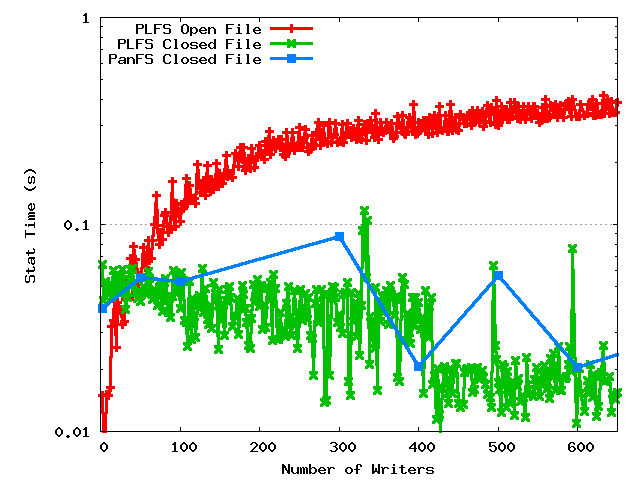
\includegraphics[width=0.4\textwidth]{data/stat/stat.eps}
    \mycaption{fig-metadata}{Metadata Queries.}{
        This graph compares the time to \syscall{stat} a 20~\GB\ file
        on \plfs\ with the time to \syscall{stat} a comparable
        file on PanFS.    
        The \yaxis, which is in logscale,
        shows the \syscall{stat} time 
        as a function of the number of writers who created that
        file.  We compare the PanFS \syscall{stat} rate to the
        \plfs\ rate for files opened for writing, and to the 
        \plfs\ rate for closed files.
        \vspace{1cm}
    }
\end{figure}


% What's up with the weird data for the stat time on an open PLFS file?
% I thought maybe it had to do with the number of subdirectories so I
% reran it with 999 subdirectories and it didn't change. Not sure now.
